\documentclass[11pt]{article}
\usepackage[a4paper,margin=0.90in]{geometry}
\usepackage{amsmath,amssymb,amsthm,mathtools}
\usepackage{booktabs,array}
\usepackage{graphicx}
\usepackage{xcolor}
\usepackage[hidelinks]{hyperref}
\hypersetup{
  pdftitle={Lossless Calibration Is Stored Memory},
  pdfauthor={Lluis Eriksson},
  pdfsubject={Topological McMillan-degree and Wigner--Smith bounds for passive quantum networks}
}
\usepackage[nameinlink,capitalise]{cleveref}
\usepackage{microtype}

\newtheorem{theorem}{Theorem}[section]
\newtheorem{proposition}[theorem]{Proposition}
\newtheorem{lemma}[theorem]{Lemma}
\newtheorem{corollary}[theorem]{Corollary}
\theoremstyle{definition}
\newtheorem{definition}[theorem]{Definition}
\newtheorem{example}[theorem]{Example}
\theoremstyle{remark}
\newtheorem{remark}[theorem]{Remark}
\newtheorem{limitation}[theorem]{Limitation}

\newcommand{\C}{\mathbb{C}}
\newcommand{\T}{\mathbb{T}}
\newcommand{\D}{\mathbb{D}}
\newcommand{\diag}{\operatorname{diag}}
\newcommand{\rank}{\operatorname{rank}}
\newcommand{\ord}{\operatorname{ord}}
\newcommand{\tr}{\operatorname{tr}}
\newcommand{\op}{\mathrm{op}}
\newcommand{\dd}{\mathrm{d}}
\newcommand{\e}{\mathrm{e}}
\newcommand{\mcdeg}{\deg_{\mathrm{McM}}}

\title{Lossless Calibration Is Stored Memory:\\
A Topological McMillan-Degree and Wigner--Smith Law\\
for Passive Quantum Networks}
\author{Lluis Eriksson}
\date{10 August 2026}

\begin{document}
\maketitle

\begin{abstract}
How many internal passive modes are required to transmit prescribed quantum
noise channels without loss while suppressing all signal directions
elsewhere?  We prove an architecture-independent answer for finite-dimensional
rational networks.  Let a causal rational inner scattering matrix
$\mathsf S$ have McMillan degree $n$, signal block $G$, and complementary loss
block $C$.  At distinct regular boundary frequencies $\zeta_j$, suppose that
$G(\zeta_j)$ is isometric on a $k_j$-dimensional input subspace.  If $G$ is a
strict contraction at one other frequency, then
\[
  \sum_j k_j\leq n.
\]
Indeed, every lossless direction lies in $\ker C(\zeta_j)$; a nonzero maximal
minor of $C$ therefore has a zero of multiplicity at least $k_j$.  Exterior
powers of a minimal Blaschke--Potapov factorization show that no minor can
have more than $n$ zeros.  The same factorization yields the exact topological
delay identity
\[
 \frac1{2\pi}\int_{-\pi}^{\pi}\tr Q(\theta)\,\dd\theta
 =\mcdeg\mathsf S=n,
 \qquad Q=-\mathrm{i}\mathsf S^*\partial_\theta\mathsf S\succeq0.
\]
Thus lossless calibration multiplicity is bounded by integrated
Wigner--Smith delay and forces peak trace delay at least $\sum_jk_j$.  The
bound is sharp for every number of ports and calibration nodes.  A Rouch\'e
version makes the zero count stable under analytic passive perturbations,
while an explicit counterexample shows why pointwise approximate calibration
alone cannot imply a degree bound.  Applied to a previously constructed
irreducible six-port reservoir filter, the law counts $3S$ calibration zeros
and proves that its degree $3S+6$ is universally optimal up to six states,
not merely optimal against reducing comparators.  Its determinant gives an
exact delay spectrum whose integral equals $3S+6$ and whose peak is
exponential.  In weak-coupling dephasing, the result turns every collection
of exactly preserved spectral directions into a compulsory passive-memory
budget.  Proofs, passive perturbations, quadrature, root audits and figures
are reproduced by the linked public repository.
\end{abstract}

\noindent\textbf{Keywords:} rational inner networks; McMillan degree;
Wigner--Smith time delay; passive quantum reservoirs; Blaschke--Potapov
factorization; transmission zeros.

\section{The question and the answer}

Passive filtering is attractive in quantum reservoir engineering because it
can reshape a bath without continuous active control.  It is nevertheless
not resource-free: a sharply selective passive response is stored in internal
modes and long dwell times.  Previous work established this trade only for a
particular scalar all-pass mechanism inside an irreducible multichannel
construction \cite{ErikssonReservoir2026}.  That left the main architectural
loophole open: could a completely different passive MIMO realization obey the
same lossless calibrations with much less memory?

The answer is no for causal finite-dimensional rational inner networks.  The
obstruction is topological rather than metric.  Exact transmission makes a
complementary loss minor vanish.  A rational inner transfer of McMillan degree
$n$ can supply at most $n$ zeros to any one minor.  The winding of its
determinant is the same integer $n$, and the corresponding phase derivative
is the trace of the Wigner--Smith lifetime matrix.  Consequently
\begin{equation}\label{eq:headline}
 \boxed{
  \text{lossless calibration charge}
  \ \leq\ \text{McMillan degree}
  \ =\ \text{integrated Wigner--Smith memory}.}
\end{equation}

The ingredients surrounding \eqref{eq:headline} are classical.  McMillan
degree originated in finite passive-network realization theory
\cite{McMillan1952}; rational lossless matrices admit finite
Blaschke--Potapov products \cite{Potapov1955,AlpayJorgensenLewkowicz2016}; and
the lifetime matrix goes back to Wigner and Smith
\cite{Wigner1955,Smith1960}.  Tangential interpolation and degree-constrained
MIMO interpolation are also mature subjects
\cite{BallKang1990,GallivanEtAl2004,BallBolotnikov2017}.  Our contribution is
the missing implication from
\emph{lossless directional calibration of a principal signal block} to a
\emph{topological degree and lifetime budget of every passive completion},
including multiplicity, sharpness and a robust analytic certificate.  We do
not claim a new factorization theorem or a new definition of time delay.

The result advances a resource-boundary programme developed across three
earlier manuscripts.  The first framed a Heisenberg cut through coherence
maintenance costs \cite{ErikssonCut2026}; the second showed a finite-degree
irreducible/reducible MIMO separation \cite{ErikssonMIMO2026}; the third
embedded that separation in a passive quantum reservoir and exposed a scalar
dwell-time price \cite{ErikssonReservoir2026}.  Here the comparator class
disappears: the lower bound applies to every rational inner architecture.

\paragraph{Contributions.}
\begin{enumerate}
 \item A calibration-charge theorem counts independent lossless directions,
 including several directions at the same frequency.
 \item A self-contained exterior-power proof bounds every minor by the full
 network's McMillan degree.
 \item An exact Wigner--Smith sum rule turns the algebraic count into an
 integrated and peak passive-memory lower bound.
 \item A $2m$-port family saturates all inequalities for arbitrary $m$ and
 any number of calibration frequencies.
 \item A Rouch\'e certificate preserves the count under passive analytic
 perturbations; a degree-one example proves that sampled approximate
 calibration alone is insufficient.
 \item The irreducible reservoir family is re-audited with all $3S$
 calibration zeros.  Its degree is $3S+6$, within an additive six states of
 the universal optimum, and its delay integral and peak are computed exactly.
\end{enumerate}

\section{Passive transfer model}

We use the unit-disc convention.  Let $\mathsf S:\D\to\C^{N\times N}$ be a
rational inner function: it is rational and analytic in $\D$, has no pole at
the boundary points under discussion, and satisfies
\begin{equation}\label{eq:inner}
 \mathsf S(\zeta)^*\mathsf S(\zeta)=I_N,
 \qquad \zeta\in\T.
\end{equation}
Pure delays $z^q$ are causal in this convention.  A minimal state-space
realization has dimension $n=\mcdeg\mathsf S$.  For square rational inner
functions this integer also equals the degree, or boundary winding, of the
scalar inner function $\det\mathsf S$.

Select $m$ signal input columns, $p$ protected output rows and the remaining
$\ell=N-p$ loss-output rows.  With irrelevant blocks suppressed, write
\begin{equation}\label{eq:partition}
 \mathsf S(z)=
 \begin{pmatrix}
   G(z)& *\\ C(z)& *
 \end{pmatrix},
 \qquad
 G(z)\in\C^{p\times m},\quad C(z)\in\C^{\ell\times m}.
\end{equation}
Column unitarity gives, on every regular boundary point,
\begin{equation}\label{eq:defect}
 G(\zeta)^*G(\zeta)+C(\zeta)^*C(\zeta)=I_m.
\end{equation}
This equality is the only quantum-network identity used in the degree
obstruction.  It is also the standard preservation law behind passive linear
quantum input--output models
\cite{GoughJames2009,GoughZhang2015,NurdinEtAl2016}.

\begin{definition}[Calibration charge]\label{def:charge}
At a regular point $\zeta\in\T$, the lossless calibration space is
\[
 E_\zeta:=\ker\!\left(I_m-G(\zeta)^*G(\zeta)\right),
 \qquad k_\zeta:=\dim E_\zeta.
\]
For distinct calibration nodes $\zeta_1,\ldots,\zeta_M$, their total charge is
$K:=\sum_{j=1}^M k_{\zeta_j}$.
\end{definition}

The definition asks only for norm preservation.  It does not require a
specified output phase, a common invariant channel, reciprocity or
commutativity.  From \eqref{eq:defect},
\begin{equation}\label{eq:kernelidentity}
 E_\zeta=\ker C(\zeta).
\end{equation}
A \emph{strict stop} is one regular point $\zeta_*$ for which
$\|G(\zeta_*)\|_{\op}<1$.  At such a point \eqref{eq:defect} makes
$C(\zeta_*)^*C(\zeta_*)$ positive definite.  In particular $\ell\geq m$ and
$C(\zeta_*)$ has full column rank.

\section{The minor-degree mechanism}

Two elementary lemmas carry the proof.  We include details because they make
the result easy to audit and expose exactly where rationality enters.

\begin{lemma}[Local nullity consumes determinant multiplicity]
\label{lem:nullity}
Let $A(z)$ be an $m\times m$ matrix holomorphic near $z_0$.  If
$\dim\ker A(z_0)\geq k$, then either $\det A\equiv0$ or
\begin{equation}\label{eq:nullityorder}
 \ord_{z_0}\det A\geq k.
\end{equation}
\end{lemma}

\begin{proof}
Choose a constant invertible input change of basis whose first $k$ columns
span a subspace of $\ker A(z_0)$.  The first $k$ columns of the transformed
matrix vanish at $z_0$, so every entry in those columns is divisible by
$z-z_0$.  Multilinearity of the determinant supplies at least $k$ factors.
Constant basis changes alter the determinant only by a nonzero constant.
\end{proof}

\begin{lemma}[Every minor inherits the full McMillan budget]
\label{lem:minordegree}
Let $\mathsf S$ be an $N\times N$ rational inner function of McMillan degree
$n$.  Every nonzero $r\times r$ minor of $\mathsf S$ has at most $n$ finite
zeros, counted with multiplicity and restricted to points where the minor is
regular.
\end{lemma}

\begin{proof}
A minimal finite Blaschke--Potapov factorization has exactly $n$ rank-one
factors \cite{AlpayJorgensenLewkowicz2016}:
\begin{equation}\label{eq:potapov}
 \mathsf S(z)=U\prod_{q=1}^{n}
 \left[I_N+\bigl(b_{a_q}(z)-1\bigr)u_qu_q^*\right],
 \quad
 b_a(z)=\frac{z-a}{1-\bar a z},quad |a|<1,
\end{equation}
where $U$ is constant unitary and $\|u_q\|=1$.  Factors with $a_q=0$
include integer delays.

Every $r\times r$ minor is an entry of the exterior-power matrix
$\bigwedge^r\mathsf S$.  On $\bigwedge^r\C^N$, a factor in
\eqref{eq:potapov} becomes
\[
 I+\bigl(b_{a_q}(z)-1\bigr)P_q,
\]
where $P_q$ is the orthogonal projection onto wedges containing $u_q$.
Thus every entry of the product has a common scalar denominator dividing
$\prod_{q=1}^n(1-\bar a_qz)$ and a numerator of degree at most $n$.
Cancellation can only lower the degree.  A nonzero entry therefore has at
most $n$ finite zeros.
\end{proof}

The exterior-power step is essential.  Expanding an $r\times r$ determinant
entry by entry would give the misleading loose count $rn$; the compound
matrix sees that each rank-one Potapov factor contributes at most one scalar
degree to any minor.

\section{Universal calibration-charge theorem}

\begin{theorem}[Lossless calibration is stored degree]
\label{thm:charge}
Let $\mathsf S$ be a causal $N\times N$ rational inner transfer of McMillan
degree $n$, partitioned as in \eqref{eq:partition}.  Let
$\zeta_1,\ldots,\zeta_M\in\T$ be distinct regular calibration nodes with
charges $k_j=\dim E_{\zeta_j}$.  If there exists a regular strict-stop point
$\zeta_*$ satisfying $\|G(\zeta_*)\|_{\op}<1$, then
\begin{equation}\label{eq:chargebound}
 K:=\sum_{j=1}^M k_j\leq \mcdeg\mathsf S=n.
\end{equation}
\end{theorem}

\begin{proof}
At the strict stop, $C(\zeta_*)$ has full column rank.  Select $m$ of its rows
whose square submatrix $C_I(\zeta_*)$ has nonzero determinant, and put
$f(z)=\det C_I(z)$.  Hence $f\not\equiv0$.

At node $\zeta_j$, \eqref{eq:kernelidentity} gives
$E_{\zeta_j}\subseteq\ker C_I(\zeta_j)$, so
$\dim\ker C_I(\zeta_j)\geq k_j$.  By Lemma~\ref{lem:nullity}, $f$ has a zero of
multiplicity at least $k_j$ there.  The nodes are distinct, whence $f$ has at
least $K$ zeros counting multiplicity.  It is an $m\times m$ minor of
$\mathsf S$, so Lemma~\ref{lem:minordegree} gives $K\leq n$.
\end{proof}

\begin{remark}[Why the strict stop is necessary]
If $G$ is isometric everywhere, then $C\equiv0$ and every loss minor vanishes
identically; a constant unitary signal route has degree zero and arbitrarily
many lossless ``calibrations.''  One strict stop certifies that the chosen
minor is not the zero function.  The theorem is therefore a selectivity law,
not a charge for transparent wiring.
\end{remark}

\begin{remark}[No hidden architecture comparator]
The proof permits arbitrary frequency-dependent channel mixing, arbitrary
constant unitary pre- and post-processing, nonreciprocal inner networks, and
any number $\ell\geq m$ of loss outputs.  It compares neither with a reducing
class nor with a fixed numerator denominator bidegree.  This is the precise
sense in which \cref{thm:charge} closes the main loophole left by the earlier
architecture separation \cite{ErikssonReservoir2026}.
\end{remark}

\section{Topological Wigner--Smith memory law}

For $\zeta=\e^{\mathrm{i}\theta}$ define the dimensionless Wigner--Smith
matrix
\begin{equation}\label{eq:Qdef}
 Q(\theta):=-\mathrm{i}\,\mathsf S(\e^{\mathrm{i}\theta})^*
 \frac{\dd}{\dd\theta}\mathsf S(\e^{\mathrm{i}\theta}).
\end{equation}
In a physical frequency variable $\omega$, multiplication by
$\dd\theta/\dd\omega$ restores units of time.  The sign in
\eqref{eq:Qdef} matches the analytic-disc convention; changing to a
$z^{-1}$ engineering convention reverses the orientation and requires the
corresponding sign change.

\begin{theorem}[Degree is Wigner--Smith phase volume]
\label{thm:sumrule}
For a causal rational inner $\mathsf S$ of McMillan degree $n$,
\begin{equation}\label{eq:sumrule}
 Q(\theta)\succeq0,
 \qquad
 \frac1{2\pi}\int_{-\pi}^{\pi}\tr Q(\theta)\,\dd\theta
 =\operatorname{wind}_{\T}\det\mathsf S=n.
\end{equation}
\end{theorem}

\begin{proof}
For a single factor
$E_q=I+(b_{a_q}-1)u_qu_q^*$ in \eqref{eq:potapov}, direct differentiation
gives a rank-one positive delay
\begin{equation}\label{eq:poisson}
 Q_{E_q}(\theta)=
 \frac{1-|a_q|^2}{|\e^{\mathrm{i}\theta}-a_q|^2}\,u_qu_q^*,
\end{equation}
whose trace integrates to $2\pi$.  If $A$ and $B$ are inner, the product rule
is
\[
 Q_{AB}=B^*Q_AB+Q_B.
\]
Positivity therefore survives the entire Potapov product, and trace
invariance under unitary conjugation makes the integrated traces add to
$2\pi n$.

Equivalently, cyclicity of trace gives
$\tr Q=-\mathrm{i}\,\partial_\theta\log\det\mathsf S$.  Each rank-one
factor has determinant $b_{a_q}$, so $\det\mathsf S$ winds $n$ times.
\end{proof}

Combining the two theorems yields the operational statement.

\begin{corollary}[Universal memory budget]
\label{cor:memory}
Under the hypotheses of \cref{thm:charge},
\begin{equation}\label{eq:memorybudget}
 K\leq n
 =\frac1{2\pi}\int_{-\pi}^{\pi}\tr Q(\theta)\,\dd\theta
 \leq \sup_\theta\tr Q(\theta).
\end{equation}
Moreover,
\begin{equation}\label{eq:properdelay}
 \sup_\theta\lambda_{\max}(Q(\theta))\geq\frac{K}{N}.
\end{equation}
Consequently a uniform proper-delay cap $Q(\theta)\preceq D I_N$ permits at
most $K\leq ND$ units of lossless calibration charge.
\end{corollary}

The lower bound concerns phase volume, not only a single resonant peak.  A
network may distribute the required memory broadly over frequency or
concentrate it into sharp long-lived modes, but it cannot remove the integral.
This distinction complements the earlier scalar stopband theorem, which
forced an exponentially high peak for one particular suppression mechanism
\cite{ErikssonReservoir2026}.

\section{Sharpness at every dimension}

The coefficient one in \eqref{eq:chargebound} cannot be improved.

\begin{proposition}[Exact saturation]
\label{prop:sharp}
For every $m,M\geq1$ there is a causal $2m$-port rational inner transfer with
$M$ distinct nodes, charge $m$ at each node, a perfect stop, and
\begin{equation}\label{eq:sharp}
 \mcdeg\mathsf S=mM=\sum_{j=1}^{M}k_j.
\end{equation}
Its Wigner--Smith trace is the constant $mM$, so the integrated bound and the
peak-trace bound are also equalities.
\end{proposition}

\begin{proof}
Let
\[
 H_m=\frac1{\sqrt2}\begin{pmatrix}I_m&I_m\\I_m&-I_m\end{pmatrix},
 \qquad
 \mathsf S_{m,M}(z)=H_m\diag(I_m,z^M I_m)H_m.
\]
Then
\begin{equation}\label{eq:sharpblocks}
 G(z)=\frac{1+z^M}{2}I_m,
 \qquad C(z)=\frac{1-z^M}{2}I_m.
\end{equation}
At every $M$th root of unity, $C=0$ and $k_j=m$.  At every solution of
$z^M=-1$, $G=0$.  Since $\det\mathsf S=z^{mM}$, its McMillan degree is $mM$.
Constant conjugation of $\diag(0,MI_m)$ gives $Q$, so $\tr Q=mM$.
\end{proof}

This saturating family is reducible and deliberately simple.  It proves that
irreducibility is not needed for the universal resource law.  Irreducibility
becomes useful for attaining strong stopband performance under richer
directional calibrations, as revisited in \cref{sec:irreducible}.

\section{What robustness is possible---and what is not}

Exact boundary equalities are experimentally idealized.  Two different
notions of robustness must be separated.

\subsection{Analytic zero-count stability}

Let $f_0$ be the nonzero loss minor selected in the proof of
\cref{thm:charge}.  Choose pairwise disjoint positively oriented Jordan
contours $\Gamma_1,\ldots,\Gamma_M$ in the complex frequency plane, avoiding
all poles, so that the interior of $\Gamma_j$ contains the calibration zero
$\zeta_j$ with multiplicity at least $k_j$.

\begin{theorem}[Rouch\'e-stable calibration charge]
\label{thm:rouche}
Let $\widetilde{\mathsf S}$ be another rational inner transfer, regular on and
inside every $\Gamma_j$, and let $\widetilde f$ denote the same loss minor. If
\begin{equation}\label{eq:rouche}
 \sup_{z\in\Gamma_j}|\widetilde f(z)-f_0(z)|
 <\inf_{z\in\Gamma_j}|f_0(z)|
 \qquad(j=1,\ldots,M),
\end{equation}
then
\begin{equation}\label{eq:robustdegree}
 \mcdeg\widetilde{\mathsf S}\geq\sum_{j=1}^{M}k_j.
\end{equation}
More generally the right side may be replaced by the total number of zeros
of $f_0$ inside the contours, counted with multiplicity.
\end{theorem}

\begin{proof}
Rouch\'e's theorem \cite{Ahlfors1979} gives the same zero count for $f_0$ and
$\widetilde f$ inside each contour.  Their interiors are disjoint, so
$\widetilde f$ has at least $\sum_jk_j$ zeros.  Apply
Lemma~\ref{lem:minordegree} to $\widetilde{\mathsf S}$.
\end{proof}

This is a robust \emph{model certificate}: it uses a rational fit or analytic
component model on small complex-frequency contours.  It does not pretend
that off-axis transfer values are direct laboratory observables.  In
practice, one fits a passive rational model to real-frequency scattering
data, propagates parameter uncertainty to \eqref{eq:rouche}, and verifies the
zero count on the model family.

\subsection{Why pointwise approximate calibration is insufficient}

\begin{proposition}[No count from unseparated approximate samples]
\label{prop:approxnogo}
Fix any integer $M$ and tolerance $\delta>0$.
There is a degree-one two-port rational inner transfer, $M$ distinct boundary
nodes, and a perfect stop such that the signal magnitude at every node is at
least $1-\delta$.
\end{proposition}

\begin{proof}
For $0<r<1$ set
\[
 b_r(z)=\frac{z-r}{1-rz},\qquad
 \mathsf S_r(z)=H_1\diag(1,b_r(z))H_1,
 \qquad G_r(z)=\frac{1+b_r(z)}2.
\]
This network has degree one and $G_r(-1)=0$.  Continuity and $G_r(1)=1$ give
an open boundary arc around $1$ on which $|G_r|\geq1-\delta$.  Select any $M$
distinct nodes in that arc.
\end{proof}

Thus a theorem depending only on the number of approximate samples is false:
the nodes may oversample one degree-one pass window.  Valid finite-tolerance
bounds need additional information---for example node separation plus a
derivative budget, or the analytic contour margin in \cref{thm:rouche}.  This
no-go prevents a common but serious overinterpretation of exact root counts.

\section{Near-optimal irreducible quantum reservoir filter}
\label{sec:irreducible}

We now apply the universal law to the explicit six-port family of
\cite{ErikssonReservoir2026}.  The purpose is not to repeat its architectural
separation, but to answer a question that paper could not: how far is its
internal dimension from the best \emph{arbitrary} passive architecture?

Fix $\alpha=9/20$ and $S\geq5$, and put
\begin{equation}\label{eq:familyb}
 r_S=1-\e^{-\alpha S},\quad
 b_r(z)=\frac{z-r}{1-rz},\quad
 B_S(z)=\eta_S b_{r_S}(z)^S,
\end{equation}
where $\eta_S=1$ for odd $S$ and $-1$ for even $S$.  Hence $B_S(-1)=-1$.
Let $\phi_g=(g-1)(1-r_S)$ for $g=0,1,2$ and $B_g=\e^{\mathrm{i}\phi_g}B_S$.
With the $3\times3$ Fourier matrix $F$, define
\begin{equation}\label{eq:mixers}
 U(z)=F\diag(1,z,z^2)F^*,\qquad
 U_{\rm rev}(z)=F\diag(z^2,z,1)F^*.
\end{equation}
The balanced interferometers and the full network are
\begin{equation}\label{eq:network}
 W_g(z)=\frac12
 \begin{pmatrix}1+B_g(z)&1-B_g(z)\\1-B_g(z)&1+B_g(z)\end{pmatrix},
 \qquad
 \mathsf S_S=\diag(U,I_3)\,W\,\diag(U_{\rm rev},I_3),
\end{equation}
where $W$ places the three $W_g$ on signal/loss port pairs.  Every factor is
inner.  The signal and loss blocks from the three signal inputs are
\begin{align}
 G_S(z)&=U(z)\diag\!\left(\frac{1+B_0(z)}2,
 \frac{1+B_1(z)}2,\frac{1+B_2(z)}2\right)U_{\rm rev}(z),
 \label{eq:GS}\\
 C_S(z)&=\diag\!\left(\frac{1-B_0(z)}2,
 \frac{1-B_1(z)}2,\frac{1-B_2(z)}2\right)U_{\rm rev}(z).
 \label{eq:CS}
\end{align}

Each scalar degree-$S$ inner function $B_g$ takes the value one at exactly
$S$ simple points of $\T$.  The three root sets are disjoint because the
phases $\phi_g$ are distinct modulo $2\pi$.  At a root $z$ of $B_g-1$, the
input direction $v_{g,z}=U(z)e_g$ is lossless and obeys
$G_S(z)v_{g,z}=z^2v_{g,z}$.  Hence the total calibration charge is
\begin{equation}\label{eq:KS}
 K_S=3S.
\end{equation}
At $z=-1$ every $|1+B_g(-1)|/2<1$, so the signal block is strictly
contractive.  The universal theorem already forces degree at least $3S$.

The realized degree is exact, not an entrywise upper bound.  Since
$\det U=\det U_{\rm rev}=z^3$ and $\det W_g=B_g$,
\begin{equation}\label{eq:dets}
 \det\mathsf S_S(z)=z^6\prod_{g=0}^{2}B_g(z),
 \qquad
 \det C_S(z)=z^3\prod_{g=0}^{2}\frac{1-B_g(z)}2.
\end{equation}
Therefore
\begin{equation}\label{eq:nearoptimal}
 \mcdeg\mathsf S_S=3S+6=K_S+6.
\end{equation}
The six-state overhead is exactly the two frequency-dependent mixers.  Thus
the same device previously proved superior to every calibrated reducing
comparator is now certified within an additive six states of the best
possible passive network of \emph{any} architecture.

The determinant also gives the complete trace delay:
\begin{equation}\label{eq:exacttrace}
 \tr Q_S(\theta)=6+3S
 \frac{1-r_S^2}{1-2r_S\cos\theta+r_S^2}.
\end{equation}
Consequently
\begin{equation}\label{eq:exactdelay}
 \frac1{2\pi}\int_{-\pi}^{\pi}\tr Q_S\,\dd\theta=3S+6,
 \qquad
 \max_\theta\tr Q_S(\theta)
 =6+3S\frac{1+r_S}{1-r_S}
 =6+3S(2\e^{\alpha S}-1).
\end{equation}
The area is the compulsory topological memory.  The exponentially high peak
is the additional price of concentrating the scalar all-pass phases sharply
enough to achieve exponential stop suppression.

\begin{figure}[htbp]
 \centering
 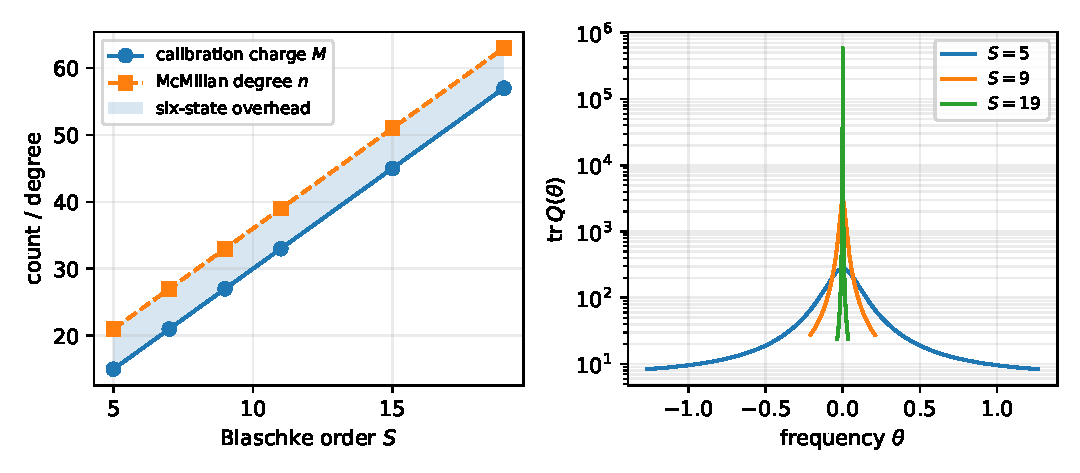
\includegraphics[width=0.94\linewidth]{figures/memory_law.pdf}
 \caption{Left: the explicit irreducible six-port construction has calibration
 charge $K_S=3S$ and exact McMillan degree $n_S=3S+6$, a constant six-state
 overhead above the universal lower bound.  Right: the same fixed phase
 volume becomes increasingly concentrated into a high Wigner--Smith peak as
 $r_S$ approaches the unit circle.  The frequency windows differ by $S$ so
 the peak shapes remain visible.}
 \label{fig:memory}
\end{figure}

\section{From scattering memory to decoherence selectivity}

The theorem is a network constraint; its quantum consequence follows through
the standard weak-coupling spectral interface.  Let a positive bath spectral
matrix obey
\begin{equation}\label{eq:bath}
 j_-I_m\preceq J(\omega)\preceq j_+I_m,
 \qquad 0<j_-\leq j_+<\infty,
\end{equation}
and define the signal contribution to a Kossakowski matrix by
\begin{equation}\label{eq:koss}
 \Gamma_G(\omega)=G(\e^{\mathrm{i}\theta(\omega)})
 J(\omega)G(\e^{\mathrm{i}\theta(\omega)})^*.
\end{equation}
This congruence is the frequency-domain form appearing in weak-coupling
Markov generators \cite{Davies1974,CerfontaineEtAl2021}.

At a calibration where $Gv=\lambda v$ with $|\lambda|=1$, contraction implies
$G^*v=\bar\lambda v$.  Hence
\begin{equation}\label{eq:passrate}
 v^*\Gamma_Gv=v^*Jv\geq j_-.
\end{equation}
At a stop where $\|G\|_{\op}\leq\varepsilon$,
\begin{equation}\label{eq:stoprate}
 \|\Gamma_G\|_{\op}\leq j_+\varepsilon^2.
\end{equation}
The spectral-rate contrast is therefore squared at the Kossakowski level.
The new statement is the compulsory resource behind preserving many pass
directions:
\begin{equation}\label{eq:quantummemory}
 \#\{\text{independent exactly preserved spectral directions}\}
 \leq \mcdeg\mathsf S
 =\frac1{2\pi}\int\tr Q.
\end{equation}

Auxiliary vacuum ports remain physical channels.  They can add a baseline to
an observed Ramsey decay, as accounted for explicitly in
\cite{ErikssonReservoir2026}; \cref{thm:charge} neither removes nor hides that
floor.  What it proves is orthogonal: regardless of how the passive network is
realized, exact preservation of $K$ selected spectral directions together
with any strict all-direction stop requires at least $K$ internal-state
degrees and the same amount of integrated delay.

This is also the precise connection to the Heisenberg-cut resource viewpoint
\cite{ErikssonCut2026}.  Active maintenance can pay in work and entropy
production; a passive architecture can avoid that continuous drive, but its
selective boundary conditions are stored as dynamical memory.  No universal
conversion from McMillan degree to joules is asserted: such a conversion
depends on linewidths, temperature, fabrication and initialization.  The
universal statement is the topological state/delay count.

\section{Reproducible certificate and adversarial checks}

The proof of \cref{thm:charge,thm:sumrule} is analytic.  Computation audits the
explicit family and deliberately probes the fragile parts of the argument.
The public repository \cite{ErikssonMemoryRepository2026} runs the following
checks.
\begin{enumerate}
 \item It generates all $3S$ closed-form calibration nodes for
 $S\in\{5,7,9,11,15,19\}$ and evaluates $\det C_S$ there.
 \item It verifies the exact determinant degrees $3S+6$ and $3S+3$ for the
 full network and selected loss minor.
 \item Adaptive quadrature checks
 $(2\pi)^{-1}\int\tr Q_S=3S+6$, including the narrow $S=19$ resonance.
 \item It checks strict nontriviality of the loss minor at the stop $z=-1$.
 \item At $S=5$, it perturbs the input and output beam-splitter angles while
 preserving passivity.  Fifteen disjoint contours are constructed around the
 reference calibration zeros.  The sampled maximum Rouch\'e ratio is below
 one, and an independent polynomial root count finds one perturbed zero in
 every contour.
 \item A fail-closed verifier rejects a missing record, incorrect degree,
 failed sum rule, trivial stop minor, non-strict Rouch\'e margin or escaped
 root.
 \item As an adversarial check of the exterior-power step, 128 seeded random
 six-port Potapov products test minors of every size from one through six and
 factor counts up to nine.  After multiplication by the single product
 denominator, every minor is fitted within the predicted polynomial degree
 budget and checked on an independent complex grid.
\end{enumerate}

\begin{table}[htbp]
\centering
\small
\begin{tabular}{@{}rrrrrr@{}}
\toprule
$S$ & charge $K_S$ & degree $n_S$ & $\frac1{2\pi}\int\tr Q_S$
& $\max\tr Q_S$ & $|\det C_S(-1)|$\\
\midrule
5  & 15 & 21 & 21.0000000000 & $2.7563\times10^2$ & 0.9972253\\
9  & 27 & 33 & 33.0000000000 & $3.0785\times10^3$ & 0.9999241\\
19 & 57 & 63 & 62.9999999909 & $5.8896\times10^5$ & 0.99999999\\
\bottomrule
\end{tabular}
\caption{Selected rows from the machine-readable certificate.  The small
$S=19$ quadrature discrepancy is below $10^{-8}$ relative error despite the
exponentially narrow delay peak.}
\label{tab:audit}
\end{table}

For the passive perturbation audit, the beam-splitter rotation is
$R(\eta)H\diag(1,B_g)HR(\xi)$ in each signal/loss pair.  The run uses angular
perturbation $2\times10^{-4}$ radians.  Across the fifteen contours the
largest sampled ratio
\begin{equation}\label{eq:rouchenumeric}
 \frac{\max_{\Gamma_j}|\widetilde f-f_0|}
 {\min_{\Gamma_j}|f_0|}
\end{equation}
is $0.04512$; every independently computed perturbed numerator has exactly
one root in each corresponding contour.  This numerical audit illustrates
\cref{thm:rouche}; the theorem itself does not depend on grid sampling.

The complete replay is:
\begin{verbatim}
python research/calibration_memory_certificate.py
python verification/verify_calibration_memory.py
\end{verbatim}
It emits
\texttt{results/calibration\_memory/certificate.json} and regenerates
\cref{fig:memory}.  The JSON file records tolerances and unrounded values.
The random-minor campaign does not replace Lemma~\ref{lem:minordegree}; it is
a falsification attempt against coding mistakes and an accidental
$rn$-rather-than-$n$ denominator count.

\section{Relation to prior theories and novelty boundary}

It is useful to separate the present statement from nearby classical results.

\paragraph{Tangential interpolation.}
General and bitangential interpolation theories ask for a rational matrix
matching prescribed directional values, often with complexity constraints
\cite{BallKang1990,BallBolotnikov2017}.  Model-reduction interpolation matches
moments or tangential transfer data \cite{GallivanEtAl2004}.  Those frameworks
do not by themselves identify the complementary loss block of a unitary
completion, turn exact norm saturation into transmission-zero multiplicity,
and equate the resulting lower bound with lifetime phase volume.

\paragraph{Blaschke--Potapov factorization.}
Potapov products describe rational inner matrices and expose their degree
\cite{Potapov1955,AlpayJorgensenLewkowicz2016}.  They are used in passive
quantum networks to separate trapped modes from propagation delays
\cite{TabakMabuchi2016}.  We use that theorem, through exterior powers, as a
sharp budget for \emph{every loss minor}; the factorization itself is not new.

\paragraph{Wigner--Smith theory.}
The lifetime matrix and total scattering phase are classical
\cite{Wigner1955,Smith1960}.  The new content is not the trace-log-determinant
identity.  It is the lower bound on that trace integral from directional
lossless calibrations of a principal block, plus its sharp realization and
passive-network consequence.

\paragraph{Earlier architecture separation.}
The previous paper proved that constant-channel reducing comparators cannot
match an irreducible construction at fixed bidegree, and obtained a scalar
peak-delay price \cite{ErikssonReservoir2026}.  The current theorem neither
assumes a reducing comparator nor uses full-spark signatures.  It certifies a
minimum full-network realization degree for every passive architecture.  The
two results are complementary: one prices architectural simplification; the
other prices lossless selectivity itself.

To the best of our knowledge after a targeted search of these literatures,
the combined calibration-charge inequality \eqref{eq:chargebound} and its
Wigner--Smith form \eqref{eq:memorybudget} have not been stated in this
passive signal/loss setting.  This is a scoped novelty claim, not a claim that
root counting, compound matrices, inner factorization or phase-delay sum
rules are individually new.

\section{Limitations and escape routes}

\begin{limitation}[Finite rational memory]
The theorem excludes singular-inner factors, ideal incommensurate distributed
delays and genuinely infinite-dimensional continua.  A finite rational
approximation has a finite McMillan degree and is covered; the convergence of
such approximations is a separate problem.
\end{limitation}

\begin{limitation}[Exact versus robust calibration]
Exact point calibration gives the clean topological charge.  Robustness is
available when an analytic contour margin is certified.  Pointwise
approximate samples alone do not suffice, by \cref{prop:approxnogo}.
Deriving optimal noisy-data bounds from separated real-frequency samples and
a measured delay cap remains open.
\end{limitation}

\begin{limitation}[Passivity]
Active gain, time variation and measurement-based feedback fall outside
rational inner scattering.  Such resources may reduce passive memory, but
they reintroduce pumping, control or entropy costs rather than refuting the
passive theorem.
\end{limitation}

\begin{limitation}[Degree is not energy]
McMillan degree and Wigner--Smith delay are architecture-independent memory
coordinates.  They do not fix fabrication volume, stored energy or
thermodynamic work without a component model.  The paper therefore does not
derive a numerical Landauer cost from \eqref{eq:chargebound}.
\end{limitation}

\begin{limitation}[Markov interface]
The decoherence interpretation uses a weak-coupling spectral generator.
Strong coupling, non-Markovian initial correlations and driven nonequilibrium
baths need a larger dynamical model.  The scattering theorem itself remains
a deterministic statement about the passive transfer.
\end{limitation}

These limitations suggest concrete next questions rather than cosmetic
extensions: a real-axis noisy-data analogue with optimal separation
dependence; an infinite-dimensional version formulated through spectral
shift; and a component-level lower bound converting delay phase volume into
stored energy or physical volume under linewidth constraints.

\section{Conclusion}

Perfect selective transmission cannot be specified for free in a passive
finite-dimensional network.  Each independent lossless direction forces a
zero of the complementary loss block; local nullity counts its multiplicity;
and a single strict stop selects a nonzero minor whose zero budget cannot
exceed the full McMillan degree.  The same integer is the winding of the
scattering determinant and the integrated Wigner--Smith lifetime.  Hence
lossless calibration is stored memory.

The inequality is coefficient-sharp, robust under an explicit analytic
Rouch\'e margin, and false under unstructured approximate sampling---all three
facts matter for a referee-proof statement.  For the irreducible six-port
reservoir construction, it upgrades an architecture-relative separation into
a universal near-optimality theorem: $3S$ calibrated directions require at
least $3S$ states, while the construction uses $3S+6$.  Its exponential
decoherence selectivity is therefore not achieved by hiding complexity in an
unpriced channel transformation.  The unavoidable memory is visible both as
topological degree and as Wigner--Smith delay.

\appendix

\section{Multiplicity at a matrix zero}

We record a coordinate-free variant of Lemma~\ref{lem:nullity}.  Let
$A(z):X\to Y$ be an analytic family between two $m$-dimensional complex
spaces.  If $\dim\ker A(z_0)=k$, select a decomposition
$X=E\oplus E^\perp$ with $E\subseteq\ker A(z_0)$ and $\dim E=k$.  In adapted
bases,
\[
 A(z)=\begin{pmatrix}
  (z-z_0)A_{11}(z)&A_{12}(z)\\
  (z-z_0)A_{21}(z)&A_{22}(z)
 \end{pmatrix},
\]
where the first block column has width $k$.  Every term in the Leibniz
formula for $\det A$ selects one entry from each of those columns and hence
contains $(z-z_0)^k$.  This proves
$\ord_{z_0}\det A\geq k$ even when the rank defect is nongeneric.  Equality
holds for a transversal zero; a higher-order degeneracy only strengthens
\cref{thm:charge}.

For the rectangular loss matrix $C:\C^m\to\C^\ell$, the strict stop gives a
set $I$ of $m$ output rows with $C_I(\zeta_*)$ invertible.  At every
calibration node, $E_\zeta\subseteq\ker C\subseteq\ker C_I$, so the same
argument applies to this single minor at all nodes.  No frequency-dependent
choice of rows is made.

\section{Exterior powers and the degree-one contribution}

For completeness, if $E(z)=I+(b(z)-1)P$ with $P=uu^*$ rank one, then
$\C^N=\operatorname{span}\{u\}\oplus u^\perp$.  Its $r$th exterior power
splits as
\[
 \bigwedge^r\C^N=
 \left(u\wedge\bigwedge^{r-1}u^\perp\right)
 \oplus \bigwedge^r u^\perp.
\]
On the first summand $\bigwedge^rE$ acts by $b(z)$; on the second it acts by
one.  Hence
\[
 \bigwedge^rE(z)=I+(b(z)-1)\Pi
\]
for a constant projection $\Pi$.  Its entries have scalar numerator and
denominator degree at most one.  A product of $n$ such matrices has a common
denominator of degree at most $n$ and entry numerators of degree at most $n$.
The coordinates of $\bigwedge^r\mathsf S$ in the standard wedge basis are
exactly the signed $r\times r$ minors of $\mathsf S$.

This also explains why the degree of a square inner matrix equals the degree
of its determinant.  For $r=N$, the exterior space is one-dimensional and
each rank-one factor contributes precisely $b_{a_q}$:
\[
 \det\mathsf S(z)=\det U\prod_{q=1}^{n}b_{a_q}(z).
\]

\section{Certificate schema and numerical conditioning}

The machine-readable ledger stores, for every $S$, the calibration
multiplicity, full-network degree, loss-minor degree, loss-zero residual,
strict-stop determinant, quadrature result, quadrature error estimate and
peak trace delay.  Closed-form phase inversion is used for calibration nodes;
high-degree polynomial root finding is intentionally avoided in the scaling
table because clustered roots near the unit circle are ill-conditioned.

Polynomial roots are used only in the $S=5$ perturbation audit, where they
serve as an independent check on the contour calculation.  The reference
contours have minimum radius $2.11\times10^{-4}$; the smallest sampled
$|f_0|$ is $2.45\times10^{-5}$ and the largest sampled perturbation is
$1.79\times10^{-6}$.  The global maximum of the per-contour ratio is smaller
than the ratio of these two global extrema and is recorded as $0.04512$.
The JSON values, rather than the rounded manuscript values, are normative for
the reproducibility test.
The same ledger records the random Potapov seed, all tested compound ranks and
the worst independent-grid interpolation residual.

\bibliographystyle{unsrt}
\bibliography{references}

\end{document}
